This section reports the end-to-end results from the updated early-window pipeline using (i) residualized structural shape descriptors, (ii) Hawkes-style dynamic parameters, and (iii) structure--tempo interaction terms. The primary analysis is conducted in size-based windows ($k \in \{10,20,30,45,60,90,120,180\}$), which hold early volume fixed by design.

\subsection{Main Performance in Size-Based Windows}
Figure~\ref{fig:k_veracity_main} and Figure~\ref{fig:k_reach_main} show the full trajectory across $k$ for veracity (AUC) and reach ($R^2$). Here, \emph{structure-only} denotes residualized structural shape features only (no tempo, dynamics, or interaction terms): this ablation isolates structural incremental signal and helps avoid treating volume effects as structure effects. At each fixed window, the gaps baseline$\rightarrow$structure-only and structure-only$\rightarrow$full/interaction-full are interpreted as incremental value from structure, then from added dynamics/interactions. The horizontal axis is window size $k$ and the vertical axis is performance (AUC or $R^2$, higher is better); colored lines are feature bundles and error bars are 95\% CIs from SE over fixed CV folds.
The headline pattern is that veracity gains are modest, while reach gains from richer bundles become clearer as $k$ increases.

\begin{figure}[htbp]
  \centering
  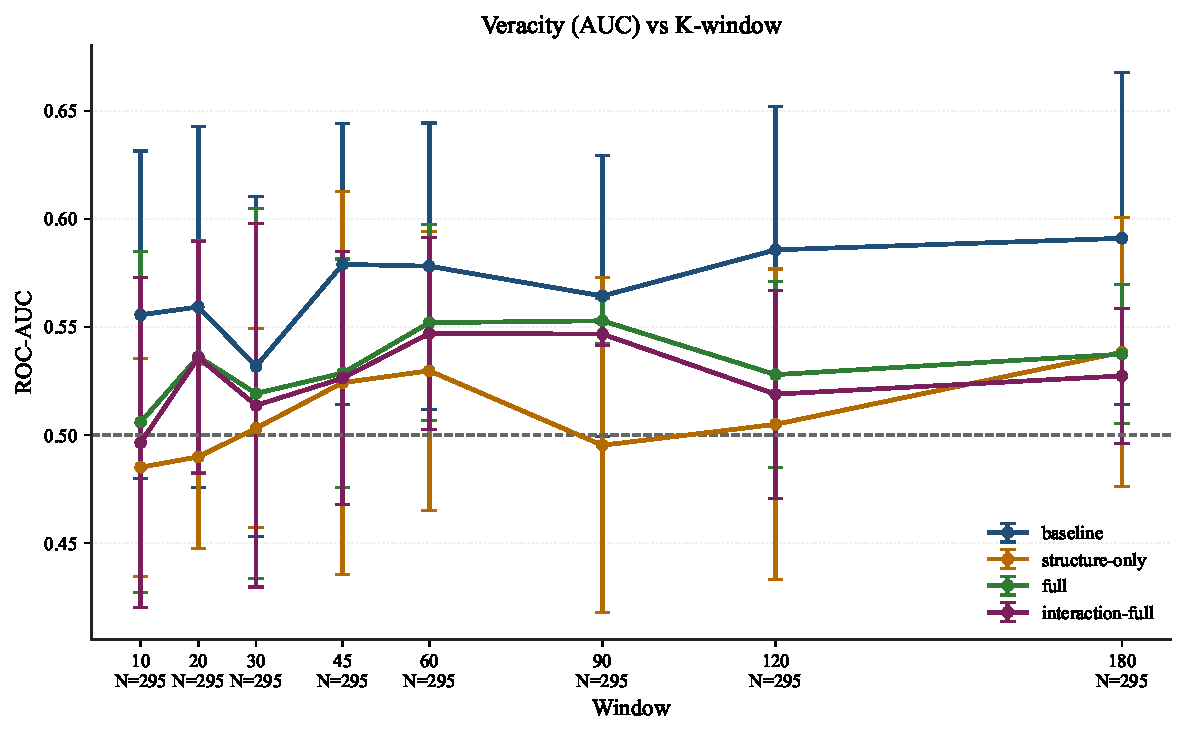
\includegraphics[width=0.8\linewidth]{Paper_sections/figures/F1K_k_veracity_primary.pdf}
  \caption{Veracity (AUC) across size-based windows. Curves compare four bundles: baseline (tempo-only), structure-only (residualized structural shape features only; no tempo, dynamics, or interactions), full (baseline + structure + dynamics), and interaction-full (full + structure--tempo interactions). Error bars are 95\% CIs (from SE over fixed CV folds).}
  \label{fig:k_veracity_main}
\end{figure}

\begin{figure}[htbp]
  \centering
  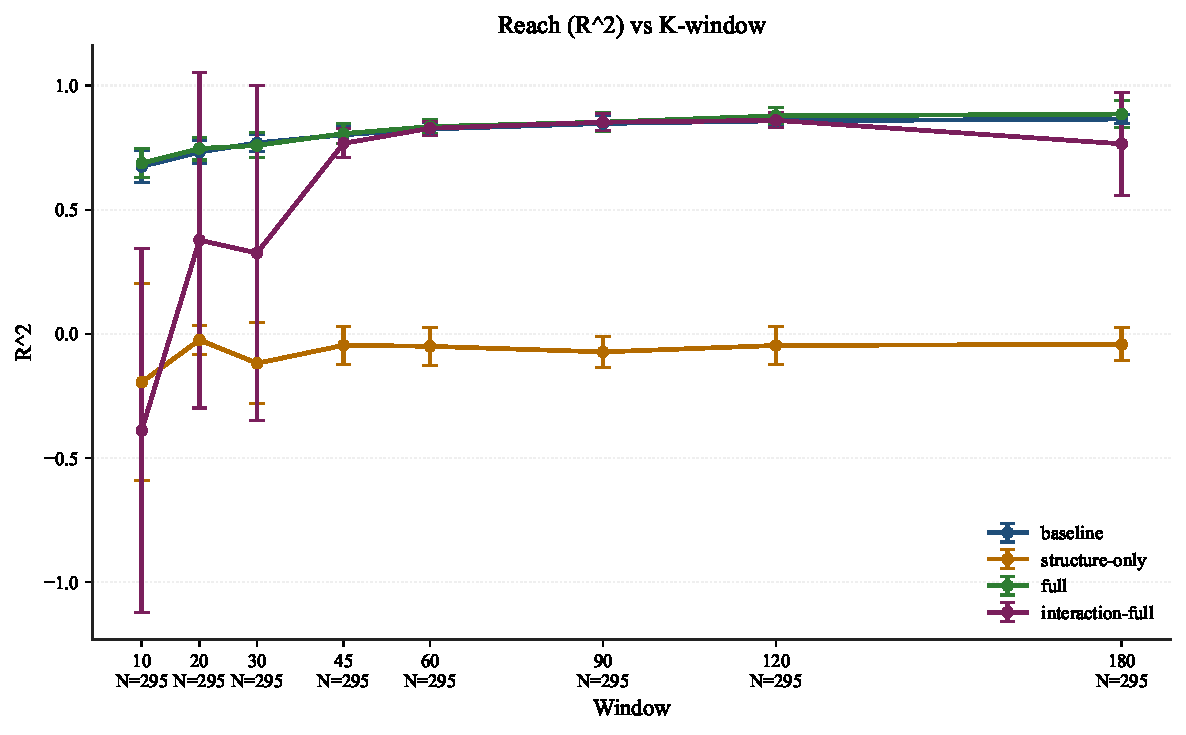
\includegraphics[width=0.8\linewidth]{Paper_sections/figures/F2K_k_reach_primary.pdf}
  \caption{Reach prediction ($R^2$) across size-based windows with the same four bundles: baseline (tempo-only), structure-only (residualized structural shape features only; no tempo, dynamics, or interactions), full (baseline + structure + dynamics), and interaction-full (full + structure--tempo interactions). Error bars are 95\% CIs (from SE over fixed CV folds).}
  \label{fig:k_reach_main}
\end{figure}

The main pattern is asymmetric across tasks. For veracity, gains from added structure/dynamics are modest under logit and strongest in early-to-mid windows (peak around $k=20$, AUC $\approx 0.657$), then flatten. For reach, improvements are limited or negative at very small windows, but become clearly positive as $k$ increases (especially from $k \ge 90$ onward).
Table~\ref{tab:k_main_selected} reports selected baseline-vs-full comparisons at representative $k$ windows.

\begin{table}[htbp]
  \centering
  \caption{Selected $k$-window comparisons: baseline vs. full feature bundle (logit for veracity, OLS for reach).}
  \label{tab:k_main_selected}
  \begin{tabular}{rrrrrrr}
    \toprule
    $k$ & AUC (baseline) & AUC (full) & $\Delta$AUC & $R^2$ (baseline) & $R^2$ (full) & $\Delta R^2$ \\
    \midrule
    10  & 0.644 & 0.646 & +0.001 & 0.010 & -0.088 & -0.098 \\
    60  & 0.634 & 0.639 & +0.005 & 0.237 & 0.286 & +0.049 \\
    120 & 0.628 & 0.621 & -0.007 & 0.402 & 0.556 & +0.155 \\
    180 & 0.609 & 0.608 & -0.002 & 0.612 & 0.719 & +0.107 \\
    \bottomrule
  \end{tabular}
\end{table}

\subsection{Model Family Comparison and Incremental Gain}
Figure~\ref{fig:model_family_k} and Figure~\ref{fig:delta_gain_k} separate model-class effects from feature-bundle effects. Figure~\ref{fig:model_family_k} compares model families under the full bundle, while Figure~\ref{fig:delta_gain_k} shows incremental gain (full minus baseline) by model family. In Figure~\ref{fig:delta_gain_k}, bars above zero ($\Delta$AUC/$\Delta R^2 > 0$) mean full outperforms baseline; bars below zero indicate the opposite. The key takeaway is that model flexibility matters more for reach than veracity, with interaction-related gains becoming clearer in later windows.
Table~\ref{tab:model_family_examples} summarizes model-family performance at representative early and late windows.

\begin{figure}[htbp]
  \centering
  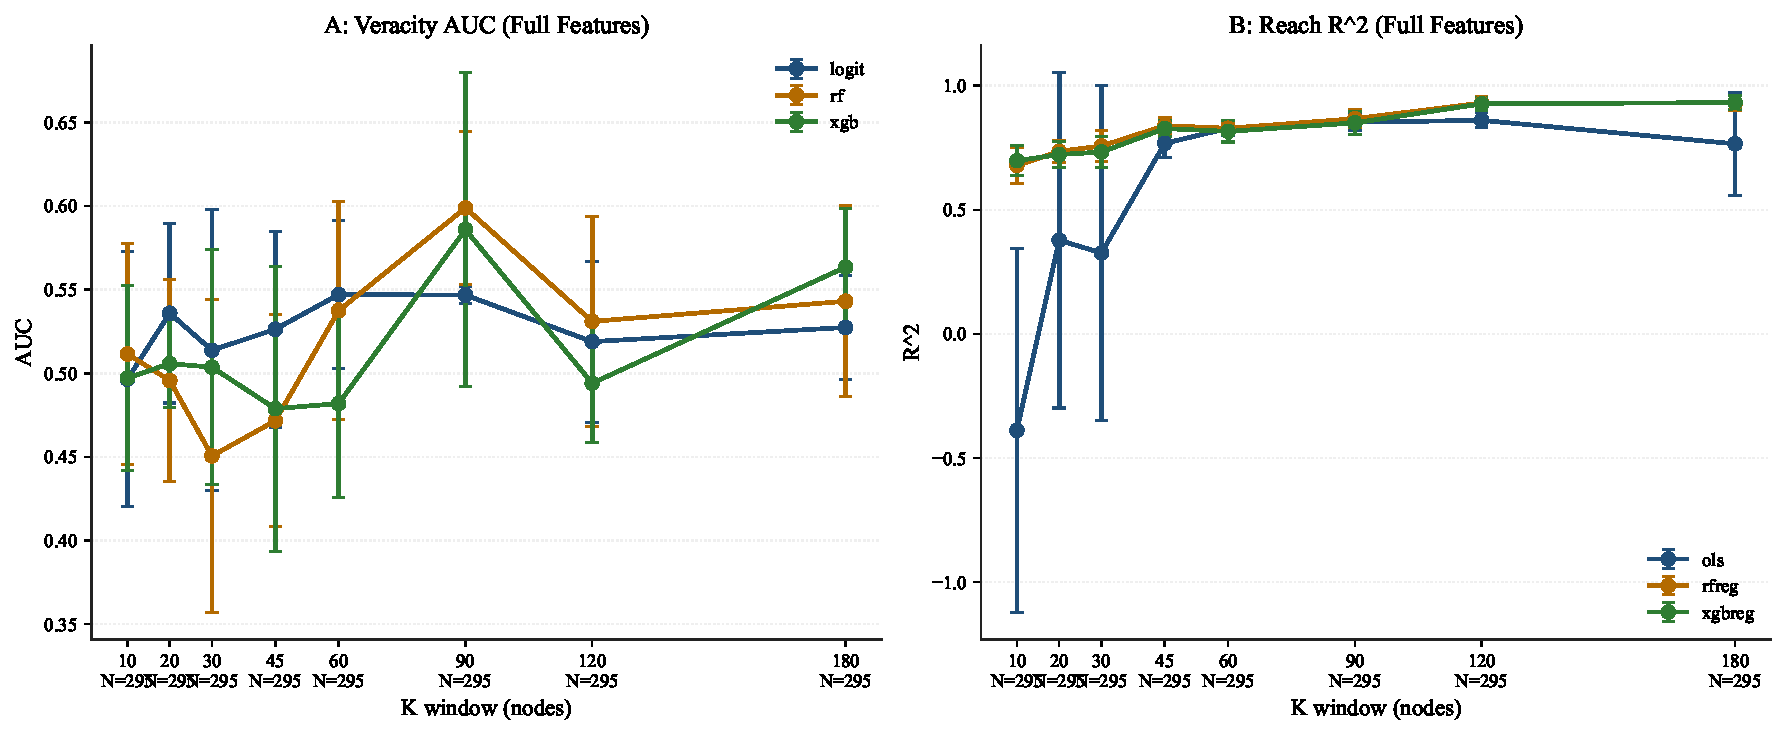
\includegraphics[width=0.95\linewidth]{Paper_sections/figures/F3_model_family_full_only.pdf}
  \caption{Model-family comparison under the full feature bundle (residualized structure + dynamics + interactions) across $k$ windows.}
  \label{fig:model_family_k}
\end{figure}

\begin{figure}[htbp]
  \centering
  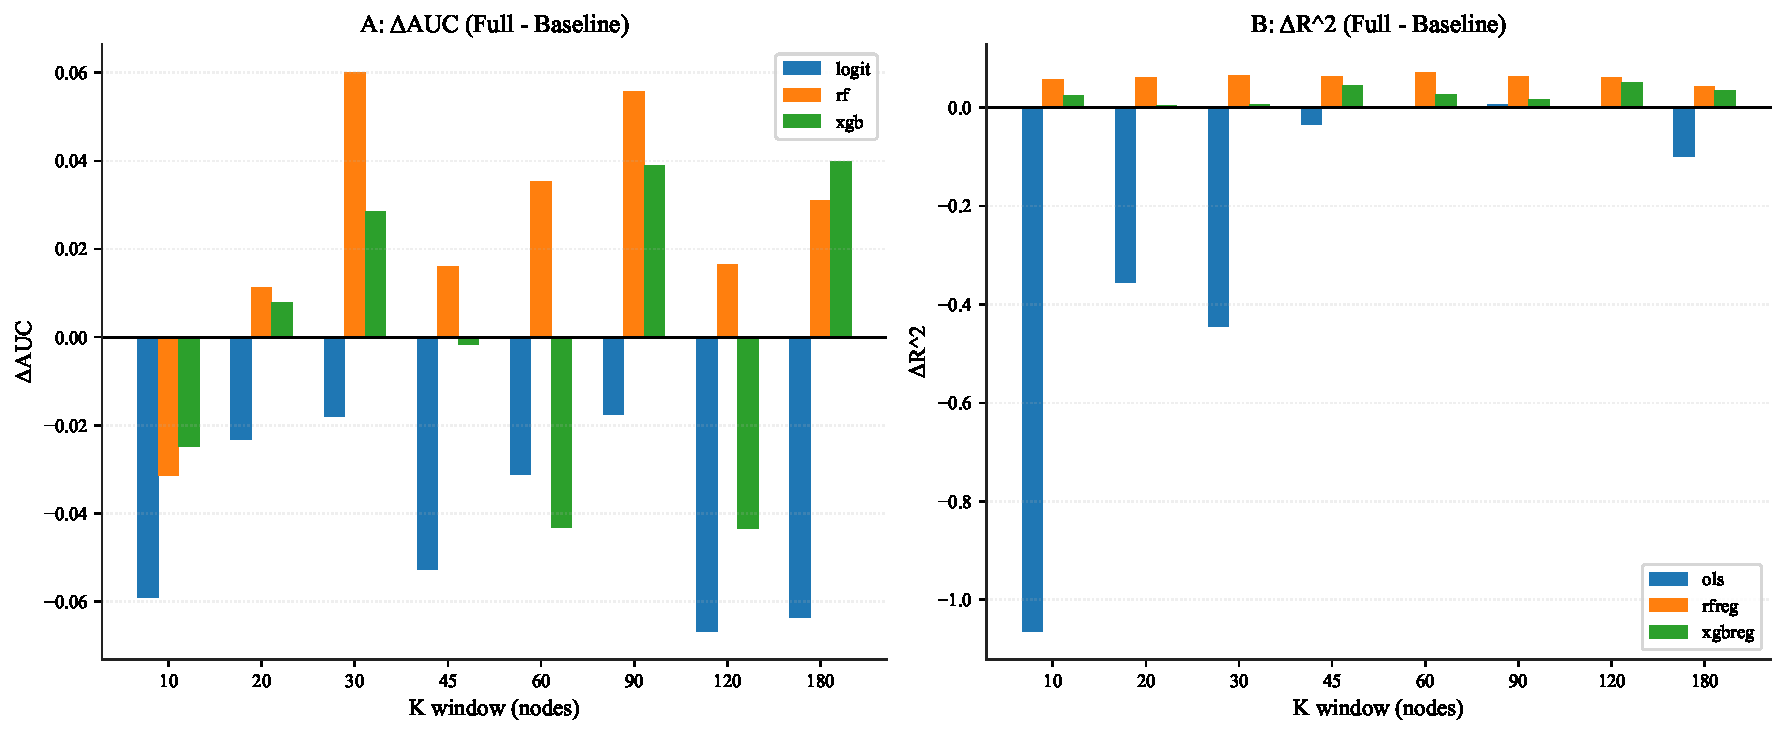
\includegraphics[width=0.95\linewidth]{Paper_sections/figures/F4_delta_gain_by_model.pdf}
  \caption{Incremental gain (full minus baseline) by model family across $k$ windows; positive bars ($\Delta$AUC/$\Delta R^2 > 0$) indicate that full improves over baseline, while negative bars indicate degradation.}
  \label{fig:delta_gain_k}
\end{figure}

\begin{table}[htbp]
  \centering
  \caption{Model-family comparison at representative early and late windows under the full feature bundle.}
  \label{tab:model_family_examples}
  \begin{tabular}{llrrrr}
    \toprule
    Window & Task & Logit/OLS & RF & XGB & Best \\
    \midrule
    $k=60$  & Veracity (AUC) & 0.640 & 0.633 & 0.623 & Logit \\
    $k=60$  & Reach ($R^2$)   & 0.254 & 0.370 & 0.345 & RF \\
    $k=180$ & Veracity (AUC) & 0.610 & 0.669 & 0.638 & RF \\
    $k=180$ & Reach ($R^2$)   & 0.719 & 0.773 & 0.772 & RF \\
    \bottomrule
  \end{tabular}
\end{table}

Two takeaways emerge. First, for veracity at small windows, linear logit remains competitive and often best, consistent with limited incremental nonlinearity at very early stages. Second, for reach, tree-based regressors dominate most windows, indicating that non-linear interactions matter more strongly for diffusion-outcome prediction than for binary veracity discrimination.

\subsection{Statistical Tests and Signal Validation}
Table~\ref{tab:k_paired_tests} reports paired fold-level $t$-tests comparing baseline vs. interaction-full models. Figure~\ref{fig:perm_k60} provides permutation-based validation at $k=60$.

\begin{table}[!htbp]
  \centering
  \caption{Paired tests (baseline vs. interaction-full): selected results from fixed 5-fold splits.}
  \label{tab:k_paired_tests}
  \begin{tabular}{rrrrr}
    \toprule
    Task & $k$ & Mean difference & $p$-value & Interpretation \\
    \midrule
    Veracity (AUC) & 45  & +0.0081 & 0.0621 & marginal \\
    Reach ($R^2$)  & 45  & -0.9175 & 0.0180 & negative early effect \\
    Reach ($R^2$)  & 90  & +0.1206 & 0.0364 & positive mid-window effect \\
    Reach ($R^2$)  & 120 & +0.1547 & $3.17\times10^{-6}$ & strong positive effect \\
    Reach ($R^2$)  & 180 & +0.1064 & $7.43\times10^{-5}$ & strong positive effect \\
    \bottomrule
  \end{tabular}
\end{table}

\begin{figure}[!htbp]
  \centering
  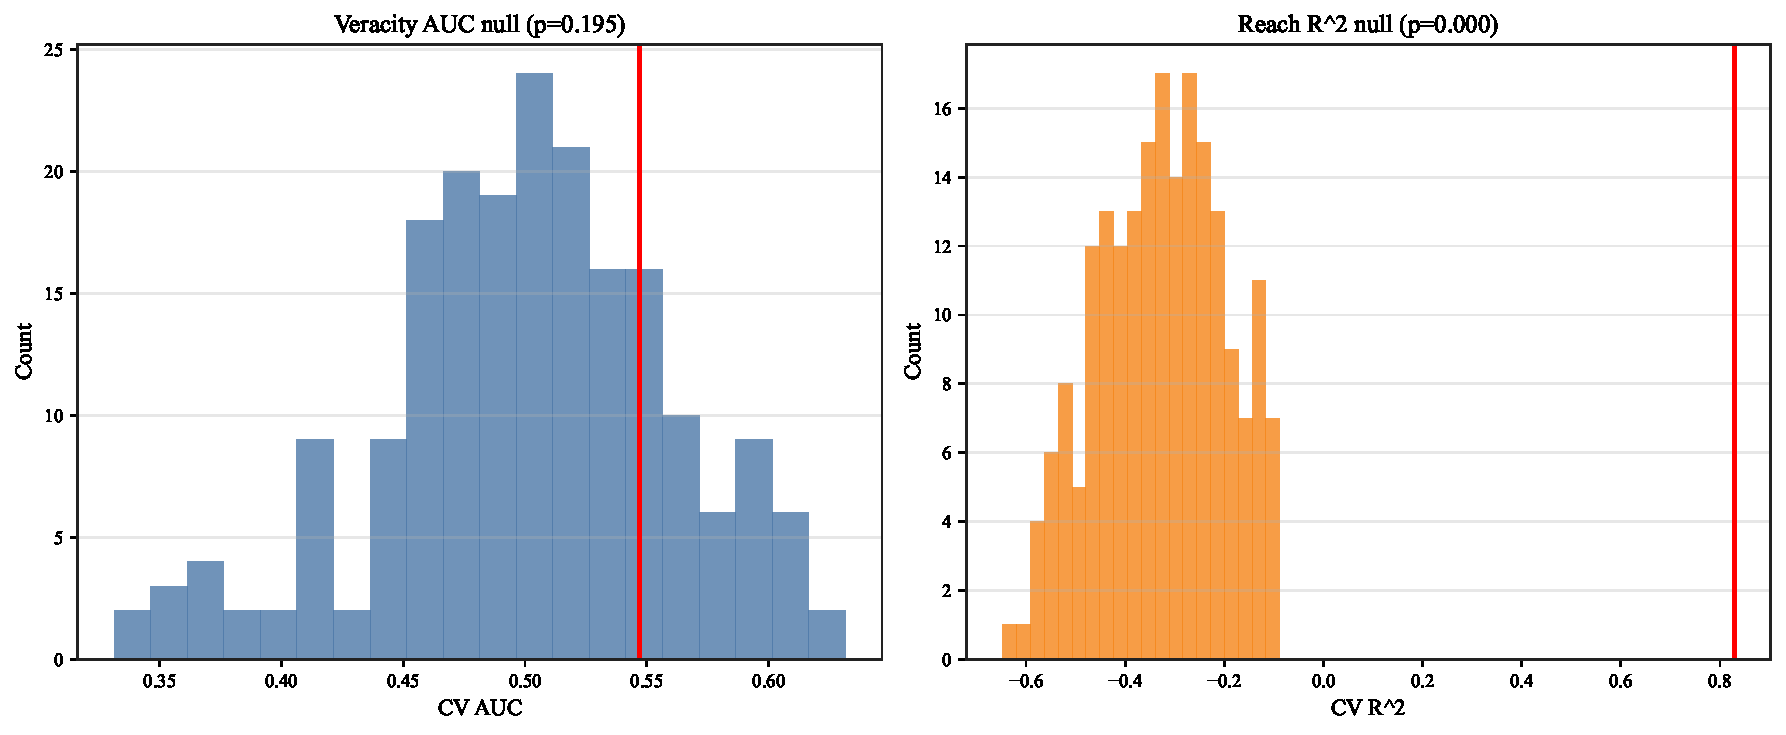
\includegraphics[width=0.88\linewidth]{Paper_sections/figures/F5_permutation_test_signal.pdf}
  \caption{Permutation tests at $k=60$ (200 shuffles). Observed scores exceed the null for both veracity (AUC) and reach ($R^2$), with empirical $p=0$.}
  \label{fig:perm_k60}
\end{figure}

Permutation results support that learned signal is non-trivial: at $k=60$, observed veracity AUC is 0.640 vs. null mean 0.499, and observed reach $R^2$ is 0.254 vs. null mean $-0.302$ (both empirical $p=0/200$).

\subsection{Supplementary Time-Window Trajectory and Feature Diagnostics}
The time-window trajectory remains useful as a secondary diagnostic (Figure~\ref{fig:time_learning_curve}), especially for showing when additional elapsed time materially improves reach prediction. The residualization diagnostics in Table~\ref{tab:residualization_diag} show that first-order dependence of structural descriptors on log early volume is effectively removed.

\begin{figure}[!htbp]
  \centering
  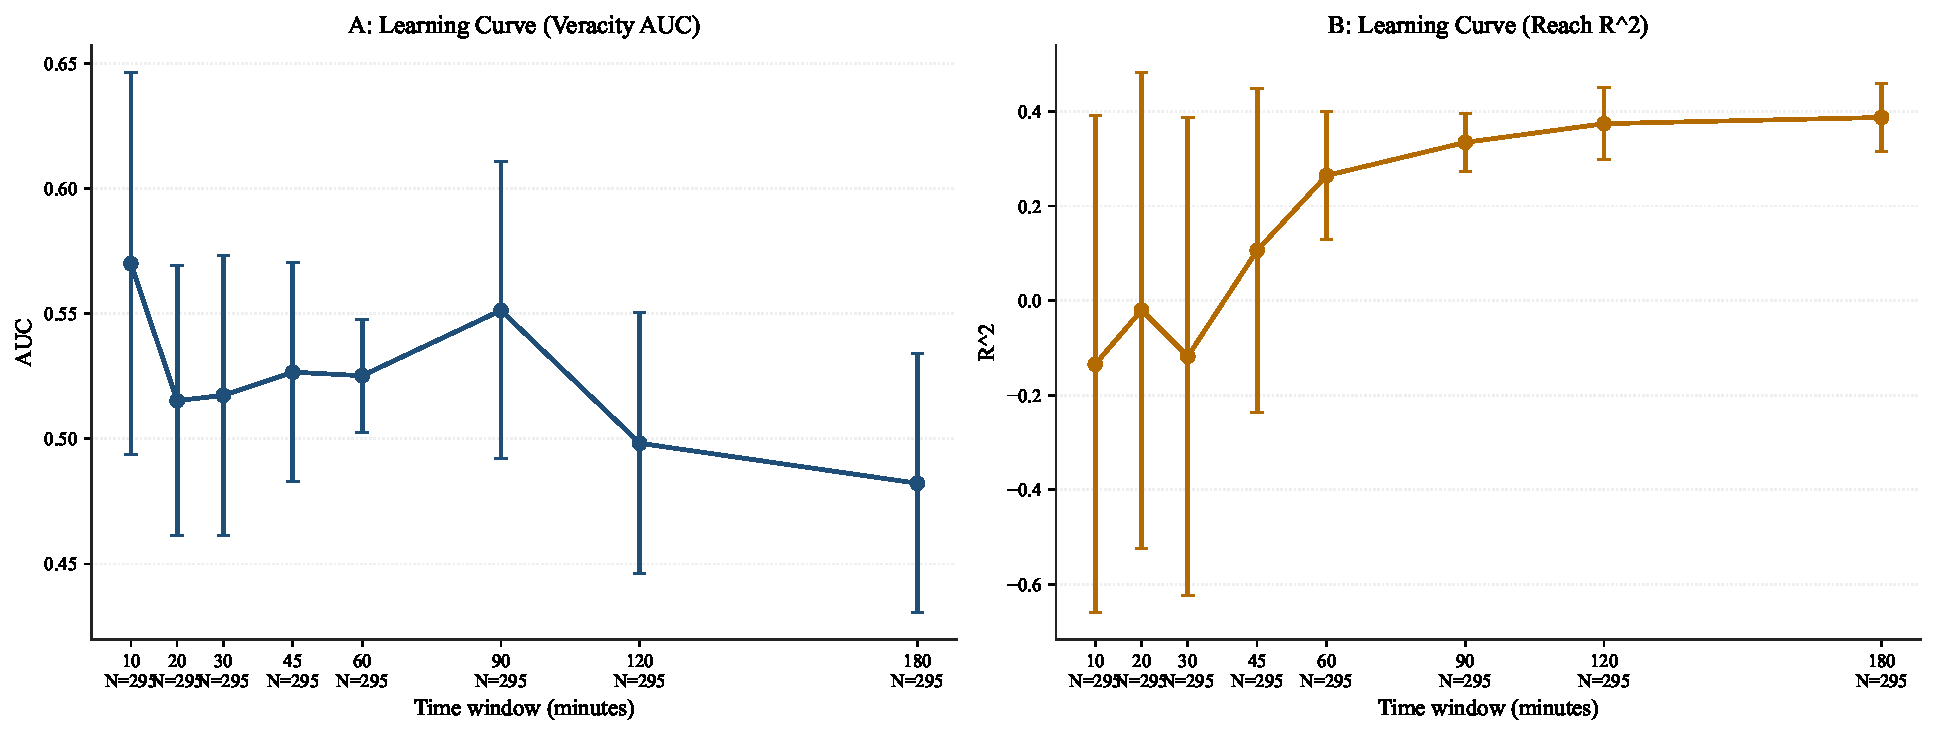
\includegraphics[width=0.92\linewidth]{Paper_sections/figures/F6_learning_curve_time.pdf}
  \caption{Supplementary time-window learning curves under the full dynamic+interaction feature bundle.}
  \label{fig:time_learning_curve}
\end{figure}

\begin{table}[!htbp]
  \centering
  \caption{Volume-dependence diagnostics before vs. after residualization (median absolute correlation with $\log(1+\text{early volume})$ over structural features).}
  \label{tab:residualization_diag}
  \begin{tabular}{lrr}
    \toprule
    Window type & Raw features & Residualized features \\
    \midrule
    Time windows & 0.248 & $\approx 3.5\times10^{-16}$ \\
    $k$ windows  & 0.103 & $\approx 1.0\times10^{-15}$ \\
    \bottomrule
  \end{tabular}
\end{table}
\FloatBarrier

\paragraph{Summary.}
Across tasks, the revised pipeline supports three conclusions: (1) size-based windows are informative and avoid confounding by raw speed; (2) residualized structural shape and dynamic interaction terms contribute more consistently to reach prediction than to veracity AUC; and (3) the strongest veracity performance appears in early-mid windows, whereas reach performance continues to improve with larger observed windows.
